%%%%%%%%%%%%%%%%%%%%%%%%%%%%%%%%%%%%%%%%%
% University Assignment Title Page 
% LaTeX Template
% Version 1.0 (27/12/12)
%
% This template has been downloaded from:
% http://www.LaTeXTemplates.com
%
% Original author:
% WikiBooks (http://en.wikibooks.org/wiki/LaTeX/Title_Creation)
%
% License:
% CC BY-NC-SA 3.0 (http://creativecommons.org/licenses/by-nc-sa/3.0/)
% 
% Instructions for using this template:
% This title page is capable of being compiled as is. This is not useful for 
% including it in another document. To do this, you have two options: 
%
% 1) Copy/paste everything between \begin{document} and \end{document} 
% starting at \begin{titlepage} and paste this into another LaTeX file where you 
% want your title page.
% OR
% 2) Remove everything outside the \begin{titlepage} and \end{titlepage} and 
% move this file to the same directory as the LaTeX file you wish to add it to. 
% Then add \input{./title_page_1.tex} to your LaTeX file where you want your
% title page.
%
%%%%%%%%%%%%%%%%%%%%%%%%%%%%%%%%%%%%%%%%%
%\title{Title page with logo}
%----------------------------------------------------------------------------------------
%	PACKAGES AND OTHER DOCUMENT CONFIGURATIONS
%----------------------------------------------------------------------------------------

\documentclass[12pt]{article}
\usepackage[portuguese]{babel}
\usepackage[utf8x]{inputenc}
\usepackage{amsmath}
\usepackage{graphicx}
\usepackage{hyperref}
\usepackage{endnotes}
\usepackage{minted}
\usepackage{tikz}
\usetikzlibrary{shapes,arrows,positioning}

\begin{document}

\begin{titlepage}

\newcommand{\HRule}{\rule{\linewidth}{0.5mm}} % Defines a new command for the horizontal lines, change thickness here

\center % Center everything on the page
 
%----------------------------------------------------------------------------------------
%	HEADING SECTIONS
%----------------------------------------------------------------------------------------

\textsc{\LARGE UFRJ}\\[1.5cm] % Name of your university/college
\textsc{\Large Telecomunicações}\\[0.5cm] % Major heading such as course name
\textsc{\large Trabalho Final}\\[0.5cm] % Minor heading such as course title

%----------------------------------------------------------------------------------------
%	TITLE SECTION
%----------------------------------------------------------------------------------------

\HRule \\[0.4cm]
{ \huge \bfseries SIGAPI\\
APIs para a UFRJ}\\[0.4cm] % Title of your document
\HRule \\[1.5cm]
 
%----------------------------------------------------------------------------------------
%	AUTHOR SECTION
%----------------------------------------------------------------------------------------

\begin{minipage}{0.4\textwidth}
\begin{center} \large
\emph{Autor}\\
Bernardo \textsc{Amorim} % Your name
\end{center}
\end{minipage}
~
\begin{minipage}{0.4\textwidth}
\begin{flushright} \large
\emph{Professor:} \\
Ph.D. Fernando Gil % Supervisor's Name
\end{flushright}
\end{minipage}\\[2cm]

% If you don't want a supervisor, uncomment the two lines below and remove the section above
%\Large \emph{Author:}\\
%John \textsc{Smith}\\[3cm] % Your name

%----------------------------------------------------------------------------------------
%	DATE SECTION
%----------------------------------------------------------------------------------------

{\large \today}\\[2cm] % Date, change the \today to a set date if you want to be precise

%----------------------------------------------------------------------------------------
%	LOGO SECTION
%----------------------------------------------------------------------------------------


\includegraphics{logo.png}\\[1cm] % Include a department/university logo - this will require the graphicx package
 
%----------------------------------------------------------------------------------------

\vfill % Fill the rest of the page with whitespace

\end{titlepage}


\begin{abstract}
This paper describes how to transform features available through UFRJ online services such as SIGA and SAP into Application Programmable Interfaces (API) so that other developers can use it to create more functionality on top of it with ease.
\end{abstract}

\section{Introdução}

O objetivo do trabalho era mostrar como é possível transformar serviços web já disponíveis em formatos para humanos em formatos para máquinas (formatos estruturados). Em especial, foram utilizados serviços da UFRJ e três serviços foram selecionados, por apresentarem características diferentes que podem demonstrar como a complexidade varia de acordo com como foi implementada a funcionalidade.

Os serviços selecionados em ordem de dificuldade são:

\begin{enumerate}
    \item Lista de Cursos e Currículos
    \item Sistema de Acompanhamento de Processos - SAP
    \item Sistema Integrado de Gestão Acadêmica - SIGA. \\
    Neste serviço foi apenas utilizada a emissão de documentos, como o Certificado de Registro em Inscrição de Disciplinas (CRID) por excemplo.
\end{enumerate}

\section{Sobre o protocolo HTTP}

Com o objetivo de deixar claro como as coisas funcionam e porque algumas medidas foram tomadas, é importante primeiro entender um pouco sobre o protocolo HTTP.

O HTTP é um protocolo pequeno e flexível, portanto deixa em aberto muitas questões sobre como se criar serviços HTTP.

\section{O WebServer e as APIs}

Todas as APIs do projeto foram feitas para exibir tudo em um formato mais bem estruturado, em JavaScript Object Notation (JSON).

Para servir os dados foi criado um servidor HTTP utilizando \textit{Node.JS}\endnote{NodeJS: \url{https://nodejs.org/}} e a biblioteca \textit{Koa.JS}\endnote{Koa.JS: \url{http://koajs.com/}}

O KoaJS serve para criar um endpoint HTTP e realizar uma ação, o arquivo \textit{index.js} realiza essa ligação (Ver anexo \ref{code:index.js})

\section{Lista de Cursos e Currículos}

A parte mais simples do trabalho foi obter a lista de cursos e seus curriculos. Por seus curriculos entenda informações sobre o curso e as disciplinas obrigatórias em cada período.

\subsection{O serviço existente}

Para utilizar como fonte de dados, utilizei uma \href{https://siga.ufrj.br/sira/repositorio-curriculo/ListaCursos.html}{página} disponibilizada no site da UFRJ.

\begin{figure}[!ht]
\centering
	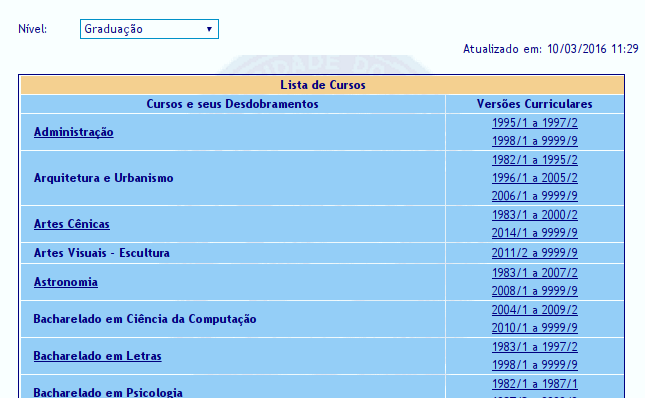
\includegraphics[width=\textwidth]{lista_cursos.png}
\caption{Página da listagem de cursos}
\label{fig:cursos}
\end{figure}

Por mais que pareça simples, na verdade essa página é consistida de outras duas páginas. Uma contem apenas a caixa de seleção do nível do curso. Esta página é responsável por carregar uma segunda página no \textit{frame} inferior.

Após escolhido o nível, é possível carregar a lista de cursos e suas especializações. Ao lado direito de cada curso existem as versões curriculares deles, que contêm cada um \href{https://siga.ufrj.br/sira/temas/zire/frameConsultas.jsp?mainPage=/repositorio-curriculo/61AD45DD-92A4-F79B-3D87-7A444052DF9B.html}{link para a página do currículo}.

A página é composta de 3 partes, um frame decorativo (removido na imagem), um separado para mostrar os detalhes do curso, e um contendo a seleção da distribuição curricular, que após abrir algumas dezenas de cursos na mão, verifiquei que apenas 1 distribuição é usada (isto fez com que, na hora de produzir a API fosse utilizada apenas a primeira).

Ela contem alguns detalhes do curso, vide Figura \ref{fig:curso}, e também as informações da distribuição curricular contem também as disciplinas do curso, conforme a figura \ref{fig:curso_periodos}.

\begin{figure}[H]
\centering
	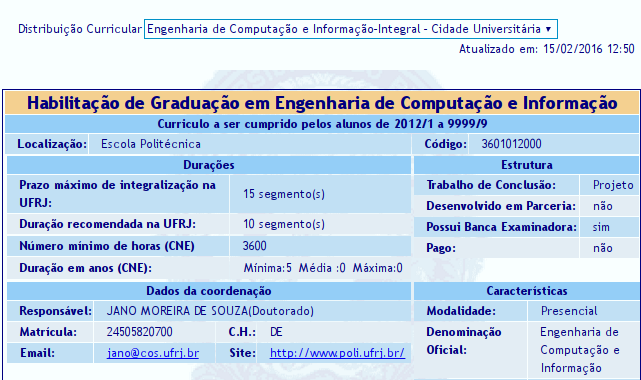
\includegraphics[width=\textwidth]{curso.png}
\caption{Página de detalhes do curso}
\label{fig:curso}
\end{figure}

\begin{figure}[H]
\centering
	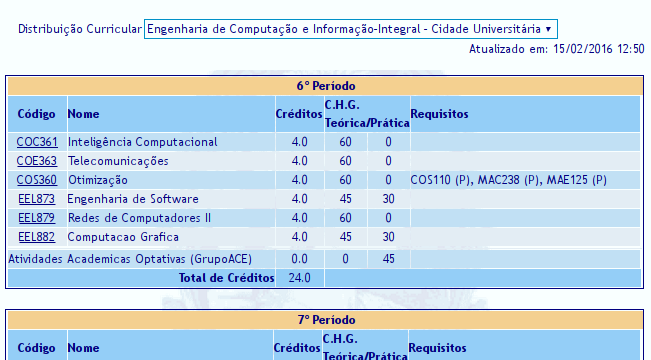
\includegraphics[width=\textwidth]{curso_periodos.png}
\caption{Disciplinas do curso}
\label{fig:curso_periodos}
\end{figure}

\subsection{Criando a API}

Primeiro foi criado um módulo \textit{curriculum.js} (Ver anexo \ref{code:curriculum.js}) contendo os seguintes métodos:

\begin{enumerate}
	\item \textit{getLevels}: Obtem os níveis de cursos (Aperfeiçoamento, Graduação, Mestrado, etc...)
	\item \textit{getCourses}: Obtém, dado um nível, os cursos disponíveis e suas especialiazções.
	\item \textit{getAllCourses}: Um método que obtem todos os níveis utilizando o \textit{getLevels} e para cada nível obtém os seus cursos.
	\item \textit{getCourse}: Dado um curso, obtém informações relevantes do curso, como orientador e disciplinas obrigatórias de cada período.
\end{enumerate}

Cada um desses métodos faz requisições HTTP para as páginas do serviço original, utiliza algumas Expressões Regulares para extrair os dados e cria um objeto JavaScript para no futuro ser convertido em \textit{JSON}.

Por último era preciso criar os \textit{endpoints} no servidor HTTP, mapeando cada um deles para uma dos métodos implementados:

\begin{enumerate}
	\item \textit{/levels/} $\Rightarrow$ \textit{getLevels}
	\item \textit{/levels/:id/courses} $\Rightarrow$ \textit{getCourses}
	\item \textit{/courses} $\Rightarrow$ \textit{getAllCourses}
	\item \textit{/courses/:id} $\Rightarrow$ \textit{getCourse}
\end{enumerate}

\begin{figure}[H]
  \centering
    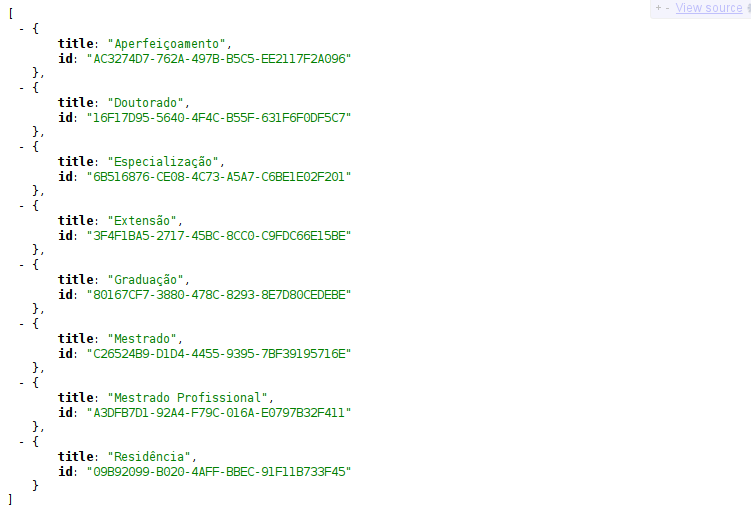
\includegraphics[width=\textwidth]{api_levels.png}
  \caption{Respostas da api de níveis}
\end{figure}
\begin{figure}[H]
  \centering
    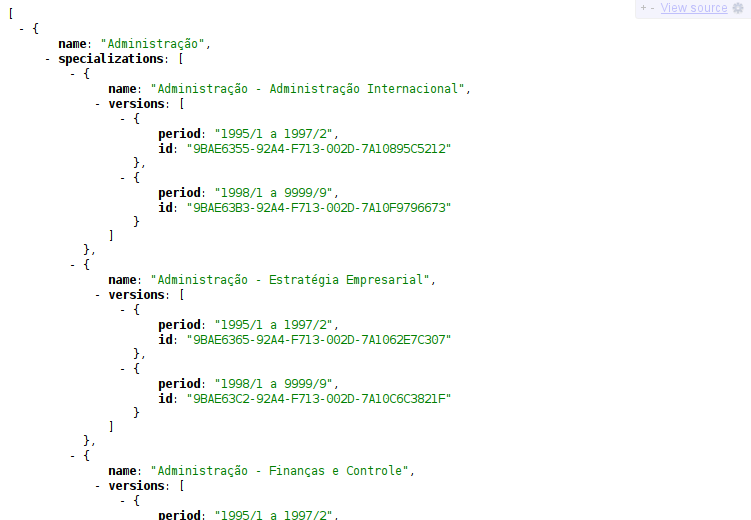
\includegraphics[width=\textwidth]{api_courses.png}
  \caption{Respostas da api de cursos}
\end{figure}
\begin{figure}[H]
  \centering
    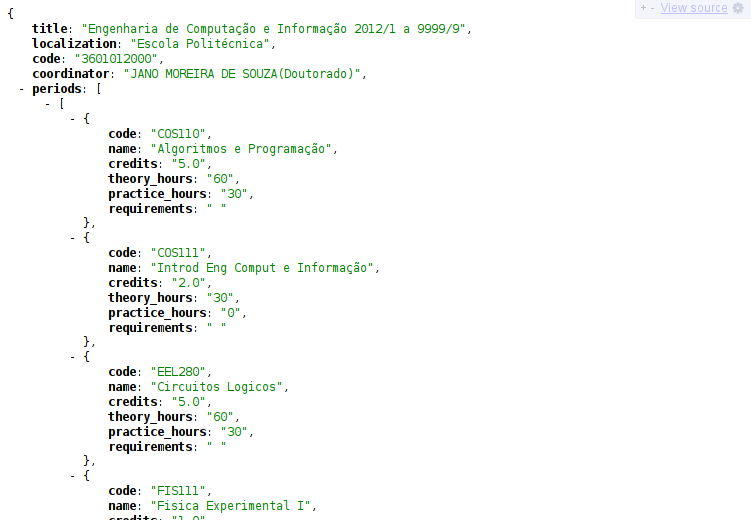
\includegraphics[width=\textwidth]{api_course.png}
  \caption{Respostas da api de curso}
\end{figure}

\section{Sistema de Acompanhamento de Processos}
O Serviço de Acompanhamento de Processos é a ferramenta online da UFRJ para que interessados possam consultar o andamento de processos dentro da faculdade, como dispensa de disciplinas e equivalência de créditos.

\subsection{O serviço existente}

O serviço consiste em duas formas de utilização: Uma é consultar direto pelo número do processo e outra permite pesquisar utilizando alguns campos (Ver figura \ref{fig:sap_pesquisa})

Ao clicar em \textit{pesquisar}, o usuário é apenas notificado de quantos resultados foram retornados e ele deve clicar em \textit{resultados}, o que leva ele a página contendo os resultados (Ver figura \ref{fig:sap_results})

\begin{figure}[!hp]
  \centering
    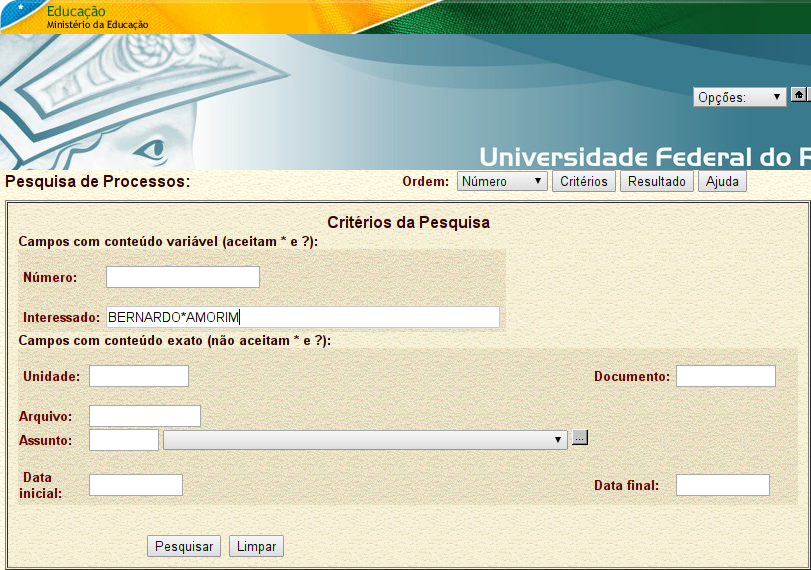
\includegraphics[width=\textwidth]{sap_pesquisa.png}
  \caption{Interface de pesquisa do SAP}
  \label{fig:sap_pesquisa}
\end{figure}

\begin{figure}[!hp]
  \centering
    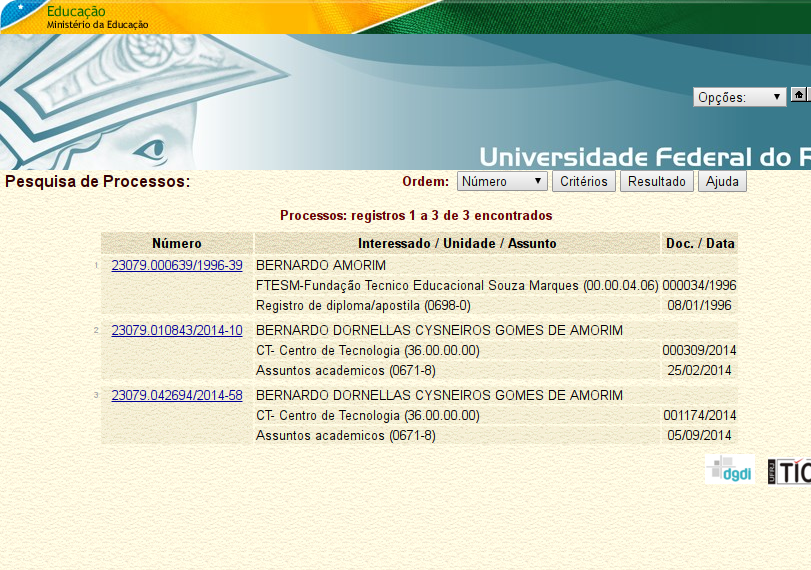
\includegraphics[width=\textwidth]{sap_results.png}
  \caption{Interface com resultados de uma pesquisa SAP}
  \label{fig:sap_results}
\end{figure}

\subsection{Criando a API}

O principal problema em criar uma API para o SAP é relacionado com ele \textbf{não} ser \textit{stateless}, isto é, ele \textbf{guarda estado} de uma página para a outra.

Ele faz isso utilizando os chamados \textit{Cookies}, e utiliza isso para guardar a ultima pesquisa. Portanto quando clicamos em \textit{pesquisar} o sistema, ao invés de pesquisar e retornar em seguida os resultados, ele guarda um estado no servidor do SAP que é lembrado ao clicarmos em \textit{resultados}.

Eles utilizam um conceito chamado \textit{sessões} e faz isso criando um cookie \textit{ASPSESSION} onde ele guarda um identificador de sessão que é guardado no servidor deles também. Portanto, quando o servidor nos retorna um header \textit{Set-Cookie} o programa deve guardar esse cookie para fazer requisições futuras.

Dado isso, o nosso programa não pode, assim como no módulo de curriculos, simplesmente fazer uma requisição pedindo os resultados. Ele deve seguir um passo a passo:

\begin{enumerate}
  \item Fazer uma requisição para \url{http://sap.ufrj.br} e obter o conteúdo do header \textit{Set-Cookie} e guardar os cookies.
  \item Utilizando os cookies obtidos, fazer uma requisição \textit{POST} para \url{http://sap.ufrj.br/pesquisarCritR.asp}
  \item Ainda utilizando os cookies obtidos, fazer uma requisição \textit{POST} para \url{http://sap.ufrj.br/pesquisarR.asp} para em fim, obter uma resposta HTML
  \item Extrair informações sobre os processos do HTML retornado.
\end{enumerate}

Portanto o módulo \textit{sap.js} foi criado (Ver anexo \ref{code:sap.js}) e ao entrar no endpoint \textit{/processes/search?q=QUERY} um JSON é obtido contendo a listagem de processos, vide figura \ref{fig:api_sap}.

\begin{figure}[H]
\centering
	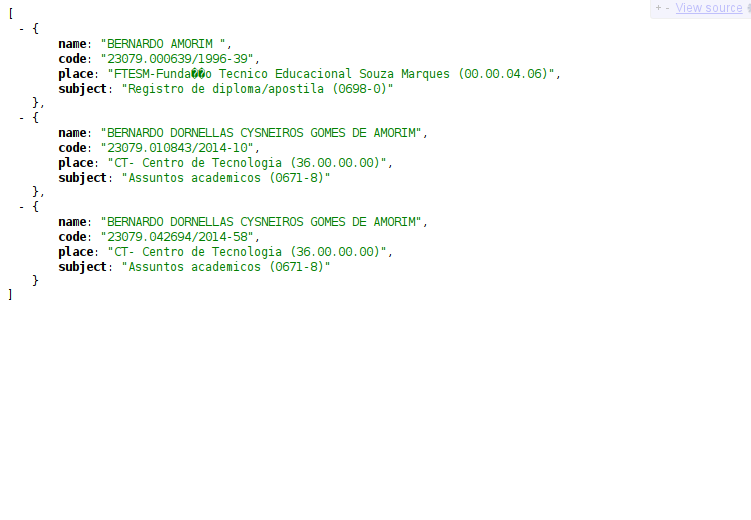
\includegraphics[width=\textwidth]{api_sap.png}
  \caption{Resposta da API do sap}
  \label{fig:api_sap}
\end{figure}

\section{SIGA e Emissão de documentos}


\subsection{O serviço existente}

Para emitir um documento, o usuário deve seguir os seguintes passos

\begin{enumerate}
  \item Fazer login utilizando CPF e senha (Ver figura \ref{fig:siga_login})
  \item Clicar na aba documentos
  \item Clicar no documento desejado (Ver figura \ref{fig:siga_documentos})
\end{enumerate}

\begin{figure}[!ht]
\centering
	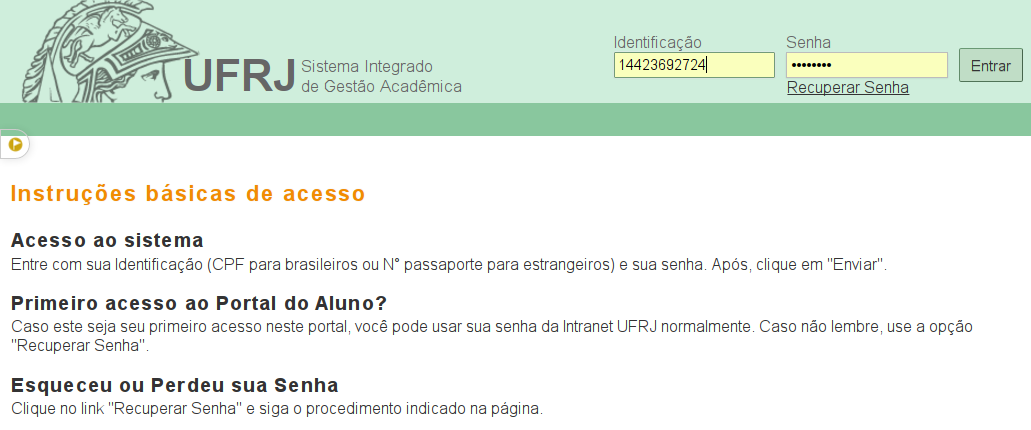
\includegraphics[width=\textwidth]{siga_login.png}
  \caption{Página de login do SIGA}
  \label{fig:siga_login}
\end{figure}

\begin{figure}[!ht]
\centering
	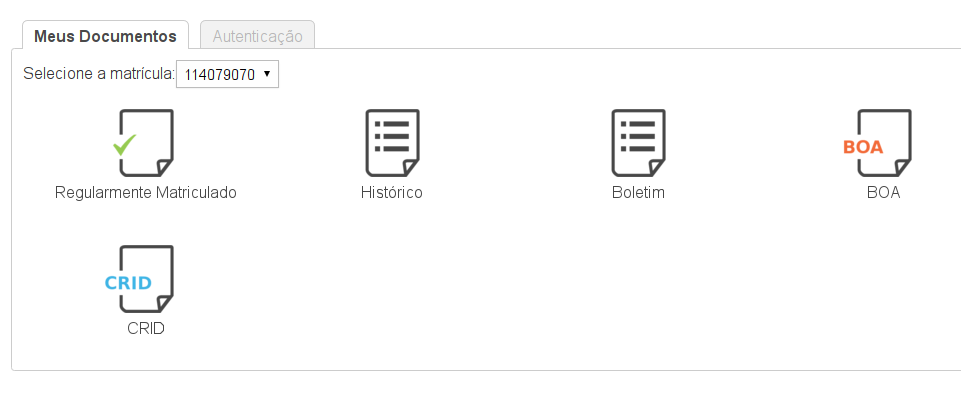
\includegraphics[width=\textwidth]{siga_documentos.png}
  \caption{Seleção de documento no SIGA}
  \label{fig:siga_documentos}
\end{figure}

\subsection{Criando a API}

Embora o uso por um usuário normal seja extremamente simples, a aplicação em sí é extremamente complicada. Basicamente porque utiliza muito código \textit{javascript} no cliente, dificultando que consigamos reproduzir o funcionamento apenas usando algumas requisições HTTP. Além disso muitas validações são feitas (provavelmente para evitar esse tipo de engenharia reversa) e essas validações tornam essa reprodução muito complicada.

Dada estas circunstâncias, um método diferente foi utilizado. Desta vez foi simulada a interação do usuário utilizando um navegador \textit{headless}, isto é, sem interface gráfica e através de um script, automatizamos as ações que um usuário normal faria para baixar um documento (as mesmas citadas acima)

Por fim este documento PDF deve ser transformado até extrairmos em formato estruturado as informações dele. Um exemplo está no diagrama abaixo:

\tikzstyle{block} = [draw, rectangle, minimum height=3em, minimum width=3em]
\tikzstyle{virtual} = [coordinate]

\begin{figure}[H]
\begin{tikzpicture}[auto, node distance=3cm]
  \node [virtual] (input1) {};
  \node [virtual, right of=input1] (input2) {};
  \node [block, below= 1cm of input2]   (browser) {Navegador};
  \node [block, right= 2cm of browser]       (pdftotext) {PDF $\Rightarrow$ Texto};
  \node [block, below=1.5cm of pdftotext]     (api) {Texto $\Rightarrow$ JSON};
  \node [virtual, right of=api]               (output) {};

  % Connect
  \draw [->] (input1) -- node {usario, senha, documento} (input2);
  \draw [->] (input2) -- node {} (browser);
  \draw [->] (browser) -- node {doc.pdf} (pdftotext);
  \draw [->] (pdftotext) -- node {doc.txt} (api);
  \draw [->] (api) -- node {JSON} (output);
\end{tikzpicture}
\caption{Diagrama do processo de obter documentos}
\end{figure}

No primeiro bloco, utilizamos como navgador o \textit{PhantomJS}\endnote{PhantomJS: \url{http://phantomjs.org/}} e além disso para tornar a criação de scripts para interagir com o navegador e facilitar o download de arquivos, foi utilizada a biblioteca \textit{CasperJS}\endnote{CasperJS: \url{http://casperjs.org/}}.

O que foi criado foi um script para o \textit{CasperJS}, o \textit{get\_documents.js} (Ver anexo \ref{code:get_documents.js}). Este script baixa um arquivo pdf contendo o documento.

Para transformar o pdf em texto, utilizei a ferramenta \textit{pdftotext}\endnote{pdftotext: \url{http://linux.die.net/man/1/pdftotext}}. Para simplificar este comportamento foi criado um shell script, o \textit{get\_documents.sh} (Ver anexo \ref{code:get_documents.sh}), que salva o PDF para um arquivo temporário e depois utiliza o \textit{pdftotext} para imprimir para a saida padrão o texto final.

Por fim, para converter o texto para um formato estruturado, foi criado o módulo \textit{documents.js} (Ver anexo \ref{code:documents.js} que para motivos de demonstração só implementava a transformação do CRID na função \textit{getCrid}.

Ao acessar o endpoint \textit{/documents/crid?username=CPF\&password=SENHA} ele obtinha um JSON contendo todas as disciplinas inscritas, vide figura \ref{fig:api_crid}.

\begin{figure}[!ht]
\centering
	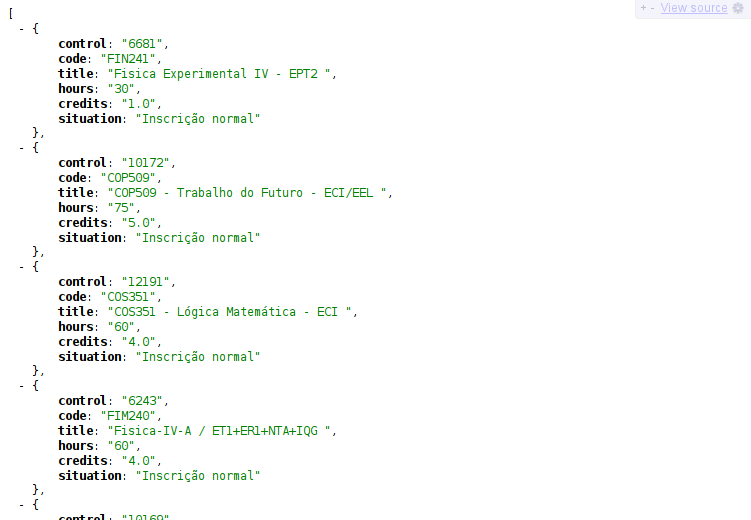
\includegraphics[width=\textwidth]{api_crid.png}
  \caption{Resposta da API do crid}
\label{fig:api_crid}
\end{figure}

\subsection{Problemas}

Tudo estava funcionando bem, até que na semana anterior a apresentação alguns eventos aconteceram:

\begin{enumerate}
  \item O SIGA saiu do ar por alumas horas.
  \item O SIGA mudou a forma como os documentos eram baixados, e essa nova forma, além de diferente (o que inutilizava o script do \textit{CasperJS}) não funcionava.
  \item O SIGA voltou com a versão antiga, mas talvez por estarmos no final do período, não dá para emitir o CRID, apenas os outros documentos.
\end{enumerate}

Dada estas circunstâncias, o que eu fiz foi utilizar um crid já baixado e conectar ele diretamente ao módulo \textit{documents.js}.

\section{Conclusão}

Embora o objetivo fosse criar bem mais APIs, o tempo tomado para algumas funcionalidades foi muito grande, principalmente pela necessidade de fazer Engenharia Reversa com muitas coisas.

No geral a experiência foi positiva e até mesmo algumas funcionalidades complicadas (como emitir documentos) foi realizada com sucesso.

O maior problema de manter APIs desta forma é que fica dependendo de os fornecedores das bases de dados originais não mudarem o serviço deles, o que aconteceu inclusive durante o andamento do projeto com as mudanças no SIGA.

Entretanto, essa é exatamente a motivação para criar essas APIs, pois caso algo mude, apenas essa caixa preta deve ser mudada, possibilitando que muitos outros desenvolvedores poupem trabalho.

Obviamente os códigos produzidos não são 100\% a prova de erros e prontos para serem colocados em produção. Eles são apenas experimentos que funcionam para casos de uso específicos, muito esforço deveria ser colocado para criar essas APIs no futuro.

Uma parte interessante que ficou faltando que foi prometida era o armazenamento de usuário e senha de forma criptografada para que a autenticação fosse feita apenas com um token, mas como a ligação com a função de obter o crid foi feita diretamente com um arquivo salvo e não sobrou muito tempo, esta funcionalidade ficou de fora.

\section{Anexos}

Todos os arquivos também podem ser encontrados no \href{https://github.com/bamorim/sigapi}{repositório do github}\endnote{Repositório no GitHub: \url{https://github.com/bamorim/sigapi}}

\subsection{index.js}
\label{code:index.js}
\inputminted[linenos]{javascript}{../sigapi/index.js}

\subsection{curriculum.js}
\label{code:curriculum.js}
\inputminted[linenos]{javascript}{../sigapi/curriculum.js}

\subsection{sap.js}
\label{code:sap.js}
\inputminted[linenos]{javascript}{../sigapi/sap.js}

\subsection{documents.js}
\label{code:documents.js}
\inputminted[linenos]{javascript}{../sigapi/documents.js}

\subsection{get\_documents.sh}
\label{code:get_documents.sh}
\inputminted[linenos]{bash}{../sigapi/scripts/get_documents.sh}

\subsection{get\_documents.js}
\label{code:get_documents.js}
\inputminted[linenos]{javascript}{../sigapi/scripts/get_documents.js}

\theendnotes

\end{document}
